%%\documentclass[a4paper,12pt,oneside]{llncs}
\documentclass[12pt,letterpaper]{article}
\usepackage[right=2cm,left=3cm,top=2cm,bottom=2cm,headsep=0cm]{geometry}

%%%%%%%%%%%%%%%%%%%%%%%%%%%%%%%%%%%%%%%%%%%%%%%%%%%%%%%%%%%
%% Juego de caracteres usado en el archivo fuente: UTF-8
\usepackage{ucs}
\usepackage[utf8x]{inputenc}

%%%%%%%%%%%%%%%%%%%%%%%%%%%%%%%%%%%%%%%%%%%%%%%%%%%%%%%%%%%
%% Juego de caracteres usado en la salida dvi
%% Otra posibilidad: \usepackage{t1enc}
\usepackage[T1]{fontenc}

%%%%%%%%%%%%%%%%%%%%%%%%%%%%%%%%%%%%%%%%%%%%%%%%%%%%%%%%%%%
%% Ajusta maergenes para a4
%\usepackage{a4wide}

%%%%%%%%%%%%%%%%%%%%%%%%%%%%%%%%%%%%%%%%%%%%%%%%%%%%%%%%%%%
%% Uso fuente postscript times, para que los ps y pdf queden y pequeños...
\usepackage{times}

%%%%%%%%%%%%%%%%%%%%%%%%%%%%%%%%%%%%%%%%%%%%%%%%%%%%%%%%%%%
%% Posibilidad de hipertexto (especialmente en pdf)
%\usepackage{hyperref}
\usepackage[bookmarks = true, colorlinks=true, linkcolor = black, citecolor = black, menucolor = black, urlcolor = black]{hyperref}

%%%%%%%%%%%%%%%%%%%%%%%%%%%%%%%%%%%%%%%%%%%%%%%%%%%%%%%%%%%
%% Graficos 
\usepackage{graphics,graphicx}

%%%%%%%%%%%%%%%%%%%%%%%%%%%%%%%%%%%%%%%%%%%%%%%%%%%%%%%%%%%
%% Ciertos caracteres "raros"...
\usepackage{latexsym}

%%%%%%%%%%%%%%%%%%%%%%%%%%%%%%%%%%%%%%%%%%%%%%%%%%%%%%%%%%%
%% Matematicas aun más fuertes (american math dociety)
\usepackage{amsmath}

%%%%%%%%%%%%%%%%%%%%%%%%%%%%%%%%%%%%%%%%%%%%%%%%%%%%%%%%%%%
\usepackage{multirow} % para las tablas
\usepackage[spanish,es-tabla]{babel}

%%%%%%%%%%%%%%%%%%%%%%%%%%%%%%%%%%%%%%%%%%%%%%%%%%%%%%%%%%%
%% Fuentes matematicas lo mas compatibles posibles con postscript (times)
%% (Esto no funciona para todos los simbolos pero reduce mucho el tamaño del
%% pdf si hay muchas matamaticas....
%\usepackage{mathptm}

%%% VARIOS:
%\usepackage{slashbox}
\usepackage{verbatim}
\usepackage{array}
\usepackage{listings}
\usepackage{multirow}

%% MARCA DE AGUA
%% Este package de "draft copy" NO funciona con pdflatex
%%\usepackage{draftcopy}
%% Este package de "draft copy" SI funciona con pdflatex
%%%\usepackage{pdfdraftcopy}
%%%%%%%%%%%%%%%%%%%%%%%%%%%%%%%%%%%%%%%%%%%%%%%%%%%%%%%%%%%
%% Indenteacion en español...
\usepackage[spanish]{babel}
\usepackage[svgnames,x11names,table]{xcolor}
\usepackage{listings}
% Para escribir código en C
% \begin{lstlisting}[language=C]
% #include <stdio.h>
% int main(int argc, char* argv[]) {
% puts("Hola mundo!");
% }
% \end{lstlisting}


\title{ModSecurity}
\author{Jesús Rodríguez Heras\\Juan Pedro Rodríguez Gracia\\Gabriel Fernando Sánchez Reina}

\begin{document}
	
	\maketitle
	\begin{abstract} %Poner esto en todas las prácticas de PCTR
		\begin{center}
			Definición de ModSecurity como firewall de aplicaciones web Open Source.
		\end{center}
	\end{abstract}
	\thispagestyle{empty}
	\newpage
	
	\tableofcontents
	\newpage
	
	%%\listoftables
	%%\newpage
	
	%%\listoffigures
	%%\newpage
	
	%%%% REAL WORK BEGINS HERE:
	
	%%Configuracion del paquete listings
	\lstset{language=bash, numbers=left, numberstyle=\tiny, numbersep=10pt, firstnumber=1, stepnumber=1, basicstyle=\small\ttfamily, tabsize=1, extendedchars=true, inputencoding=latin1}


\section{ModSecurity}
\subsection{¿Qué es?}
Es un motor de detección y prevención de intrusión de código abierto (Open Source) para aplicaciones web.\\

Es un firewall de aplicaciones web que ejecuta como módulo del servidor web Apache. Provee protección contra diversos ataques web y permite monitorizar el tráfico HTTP(S), así como realizar análisis en tiempo real sin necesidad de hacer cambios en la estructura existente.\\

También provee un lenguaje de reglas y una API para implementar protecciones avanzadas. Esto significa que es posible filtrar tráfico HTTP(S), directamente en el servidor web, según el contenido de las peticiones de los clientes, lo cual permite detectar y bloquear ataques de tipo XSS (Cross Site Scripting)\footnote{Del inglés Cross-site scripting es un tipo de inseguridad informática o agujero de seguridad típico de las aplicaciones Web, que permite a una tercera persona inyectar, en páginas web visitadas por el usuario, código JavaScript o en otro lenguaje similar (por ejemplo: VBScript), evitando medidas de control como la Política del mismo origen.}, SQLi (SQL injection)\footnote{Es un método de infiltración de código intruso que se vale de una vulnerabilidad informática presente en una aplicación en el nivel de validación de las entradas para realizar operaciones sobre una base de datos.}, etc.\\

Es un producto desarrollado por Breach Security y está disponible como Software Libre bajo la licencia GNU General Public License. A su vez, se encuentra disponbible bajo diversas licencias comerciales.

\subsection{Características principales}
Las características principales de ModSecurity son su capacidad de log y filtrado lo que permite almacenar el detalle de cada petición en un archivo de log, incluyendo los ``payloads'' de los POST HTTP. Los pedidos entrantes, a su vez, pueden ser analizados, y los pedidos ofensivos, serán rechazados (o simplemente registrados en el log, de acuerdo a cómo se configure). Esto nos permite que se ejecuten aplicaciones inseguras en nuestros servidores web ya que están siendo protegidas por ModSecurity.


\section{Un poco de historia}
ModSecurity fue creado por Ivan Ristic\footnote{Especialista en seguridad web y autor de ModSecurity.} en el año 2002. El señor Ristic abordó del desarrollo de esta aplicación después de haber utilizado durante un año y medio el SNORT\footnote{Sistema de detección de intrusos en red libre y gratuito. Ofrece la capacidad de almacenamiento de bitácoras en archivos de texto y en bases de datos abiertas, como MySQL. Implementa un motor de detección de ataques y escaneo de puertos que permite registrar, aletar y responder ante cualquier anomalía previamente definida.} para monitorear el trafico web y llegar a la conclusión de que necesitaba una herramienta que le permmitiera especificar reglas más complejas y la capacidadd de realizar acciones relacionadas específicamente con el tráfico HTTP.\\

En septiempre de 2006 Breach Security\footnote{Fundada en 2004, fue el proveedor líder de seguridad e integridad de aplicaciones web continuas en tiempo real que protege la información confidencial basada en la web.} adquirió ModSecurity y fue a partir de este momento, donde el desarrollo de ModSecurity paso a llevarlo a cabo Breach Security.

\section{Implementación}
%Aquí hay una guía de la implementación de ModSecurity: https://www.seguridad.unam.mx/historico/documento/index.html-id=1083
%Una vez mirada la guía a fondo, exponer las decisiones tomadas y poner también capturas de la instalación y configuración para que, en teoría, funcione y probar si verdaderamente funciona.
%Intentar hacerlo en la máquina virtual a ver si funciona, y si no funciona, poner todos los pasos seguidos y detalladamente explicados porque Jose Antonio dijo que lo implementaramos si podíamos.
Para la implementación de ModSecurity, debemos contar con un servidor web Debian con Apache instalado y condigurado, en funcionamiento.
\subsection{Instalación y configuración de Apache en Debian.}
Con el comando ``\texttt{sudo apt-get install apache2}'' instalamos los archivos necesarios para que funcione nuestro servidor web.\\

El archivo de configuración de apache2 se encuentra en la carpeta ``\texttt{/etc/apache2}''. En el archivo principal de condiguración, ``\texttt{apache2.conf}'' lo editaremos y añadiremos el siguiente parámetro: ``\texttt{ServerName www.trabajoASRC.com}''.\\

A continuación, vamos a cambiar el nombre de dominio de nuestro servidor web. Para ello, con el comando ``\texttt{ifconfig}'' encontramos que nuestra IP es \texttt{10.0.2.15}. Ahora, editamos el archivo ``\texttt{/etc/hosts}'' incluyendo nuestra IP (\texttt{10.0.2.15}) y la entrada de nuestro servidor ``\texttt{www.trabajoASRC.com}''.\\

Para arrancar el servidor, introducimos el siguiente comando: ``\texttt{/etc/init.d/apache2 restart}''. Si queremos pararlo, solo tenemos que introducir el comando ``\texttt{/etc/init.d/apache2 stop}''.\\

Tras ejecutar el comando de inicio del servidor, nos dirigimos al navegado, introducimos la dirección de nuestro servidor web ``\texttt{www.trabajoASRC.com}'' y se nos muestra la siguiente pantalla:
\newpage
\begin{center}
	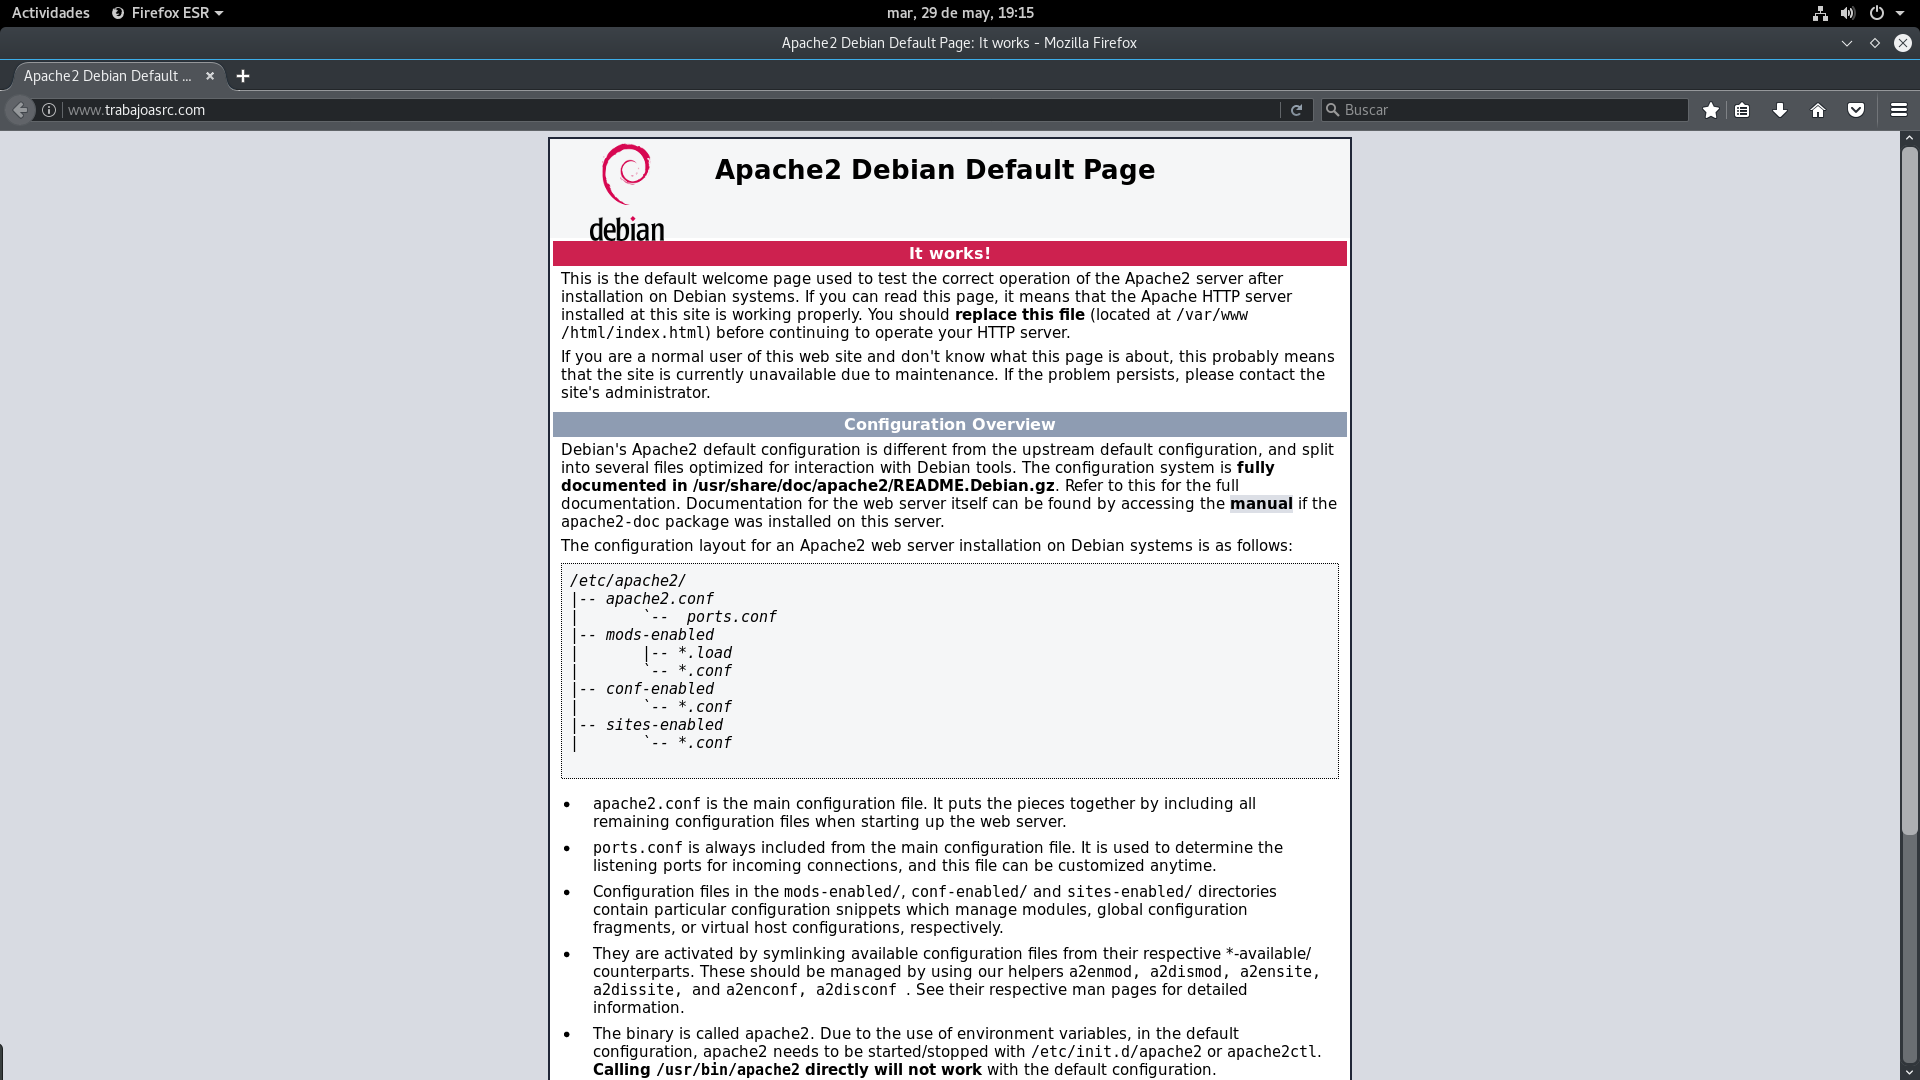
\includegraphics[scale=0.24]{apache.png}
\end{center}


\subsection{Instalación y configuración de Apache ModSecurity}
Con el comando ``\texttt{apt-get install libapache2-modsecurity}'' instalamos los paquetes necesarios para la correcta instalación de ModSecurity. Tal como se ha mencionado anteriormente, ModSecurity trabaja utilizando reglas para la detección y filtrado de diferentes tipos de ataques, las cuales se definen utilizando un lenguaje propio. Por defecto incluye un conjunto de reglas genéricas mantenidas por la comunidad OWASP\footnote{Acrónimo de Open Web Application Security Project, (en inglés ‘Proyecto abierto de seguridad de aplicaciones web’) es un proyecto de código abierto dedicado a determinar y combatir las causas que hacen que el software sea inseguro. La Fundación OWASP es un organismo sin ánimo de lucro que apoya y gestiona los proyectos e infraestructura de OWASP. La comunidad OWASP está formada por empresas, organizaciones educativas y particulares de todo mundo.}, las cuales son liberadas de manera gratuita y protegen contra los ataques básicos.\\

A continuación, nos dirigimos a ``\texttt{/etc/modsecurity}'' y encontraremos el archivo\\``\texttt{modsecurity.conf-recommended}''. Para poder trabajar con él sin perder los datos, realizamos una copia con el comando ``\texttt{cp modsecurity.conf-recommended}\\\texttt{ modsecurity.conf}'', que nos creará el archivo de configuración de ModSecurity.\\

Una vez configurado ModSecurity, tal como se indica aquí: (\url{https://samhobbs.co.uk/2016/03/getting-started-apache-modsecurity-debian-and-ubuntu}).\\

A partir de aquí, tendríamos configurado nuestro servidor de Apache con ModSecurity activado pero, por falta de conocimientos y de técnica, no hemos podido seguir adelante con la implementación. Lo que sí hemos conseguido es recolectar algunas de las reglas de ModSecurity que se muestran a continuación:
\newpage
\begin{center}
	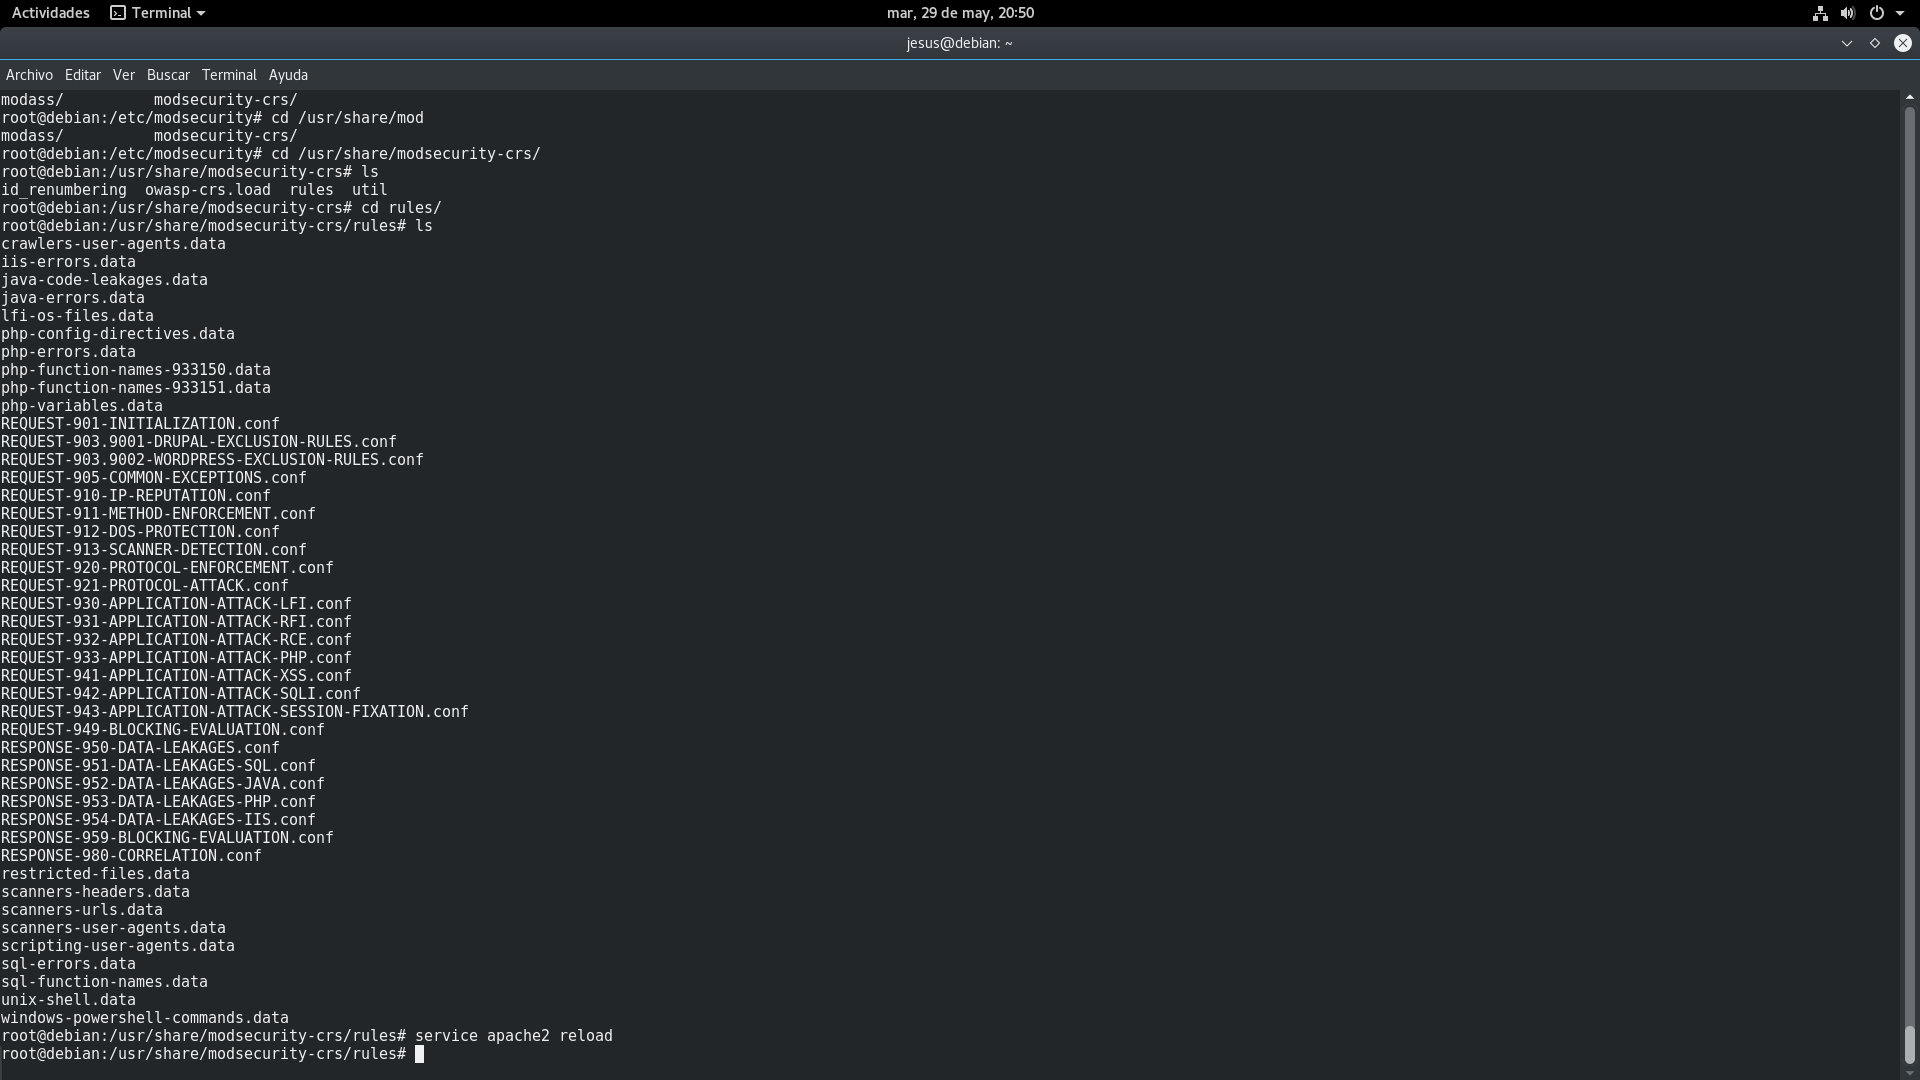
\includegraphics[scale=0.24]{reglas.png}
\end{center}

\section{Referencias}
\begin{itemize}
	\item \url{https://es.wikipedia.org/wiki/Mod_Security}
	\item \url{https://www.modsecurity.org/}
	\item \url{https://es.wikipedia.org/wiki/Inyecci\%C3\%B3n_SQL}
	\item \url{https://es.wikipedia.org/wiki/Cross-site_scripting}
	\item \url{https://blog.ivanristic.com/2006/09/modsecurity-has-been-acquired.html}
	\item \url{http://www.ite.educacion.es/formacion/materiales/85/cd/linux/m3/instalacin_y_configuracin_de_apache.html}
	\item \url{https://www.linuxito.com/seguridad/562-como-instalar-y-configurar-}\\\url{modsecurity-en-apache-sobre-servidores-debian}
	\item \url{https://es.wikipedia.org/wiki/Open_Web_Application_Security_Project}
	\item \url{https://samhobbs.co.uk/2016/03/getting-started-apache-modsecurity-}\\\url{debian-and-ubuntu}
\end{itemize}

\end{document}